\documentclass[12pt,a4paper,oneside]{report}

\usepackage[a4paper,top=2.5cm,bottom=2.5cm,left=3cm,right=2cm]{geometry}
\usepackage{fontspec}
\usepackage{graphicx}
\usepackage{xcolor}
\usepackage{array}
\usepackage{booktabs}
\usepackage{longtable}
\usepackage{tabularx}
\usepackage{multirow}
\usepackage{enumitem}
\usepackage{fancyhdr}
\usepackage{titlesec}
\usepackage{hyperref}
\usepackage{listings}
\usepackage{tikz}
\usetikzlibrary{arrows.meta,positioning,fit,shapes.geometric,calc}

\setmainfont{TeX Gyre Termes}
\setsansfont{TeX Gyre Heros}
\setmonofont{DejaVu Sans Mono}
\XeTeXlinebreaklocale "vi"
\XeTeXlinebreakskip = 0pt plus 1pt

\definecolor{TryOpsNavy}{HTML}{0F172A}
\definecolor{TryOpsBlue}{HTML}{2563EB}
\definecolor{TryOpsTeal}{HTML}{0F766E}
\definecolor{TryOpsGold}{HTML}{B45309}
\definecolor{TryOpsRed}{HTML}{B91C1C}
\definecolor{TryOpsSlate}{HTML}{475569}
\definecolor{TryOpsMist}{HTML}{F8FAFC}
\definecolor{TryOpsLine}{HTML}{CBD5E1}
\definecolor{CodeBg}{HTML}{F8FAFC}

\hypersetup{
  colorlinks=true,
  linkcolor=TryOpsBlue,
  urlcolor=TryOpsTeal,
  citecolor=TryOpsBlue,
  pdftitle={TryOps: Nen tang MLOps doanh nghiep cho VTON va LLM},
  pdfauthor={Nguyen Tran Nhat Trung, Hoang Minh Thai, Pham Hai Dang}
}

\pagestyle{fancy}
\fancyhf{}
\lhead{\small TryOps MLOps}
\rhead{\small Báo cáo đồ án cuối kỳ}
\cfoot{\thepage}
\renewcommand{\headrulewidth}{0.4pt}

\titleformat{\chapter}
  {\normalfont\huge\bfseries\color{TryOpsNavy}}
  {CHƯƠNG \thechapter.}{0.8em}{}
\titleformat{\section}
  {\normalfont\Large\bfseries\color{TryOpsNavy}}
  {\thesection}{0.7em}{}
\titleformat{\subsection}
  {\normalfont\large\bfseries\color{TryOpsBlue}}
  {\thesubsection}{0.6em}{}

\setlist[itemize]{leftmargin=1.2cm,itemsep=0.2em,topsep=0.25em}
\setlist[enumerate]{leftmargin=1.2cm,itemsep=0.2em,topsep=0.25em}
\renewcommand{\arraystretch}{1.25}
\setlength{\parindent}{0pt}
\setlength{\parskip}{0.55em}

\newcommand{\code}[1]{\texttt{\detokenize{#1}}}
\newcommand{\reporttitle}{TryOps: Nền tảng MLOps doanh nghiệp cho Virtual Try-On và phục vụ LLM hiệu quả}
\newcommand{\reportsubtitle}{Evidence Gates, Native Control Plane, Real Model Serving, Observability}

\lstdefinestyle{tryopscode}{
  basicstyle=\small\ttfamily,
  backgroundcolor=\color{CodeBg},
  frame=single,
  rulecolor=\color{TryOpsLine},
  breaklines=true,
  columns=fullflexible,
  keepspaces=true,
  showstringspaces=false,
  tabsize=2
}
\lstset{style=tryopscode}

\newcommand{\pill}[2]{%
  \tikz[baseline=-0.55ex]\node[
    fill=#1!12,
    draw=#1!35,
    text=#1,
    rounded corners=3pt,
    inner xsep=6pt,
    inner ysep=2.5pt
  ]{\scriptsize\bfseries #2};%
}

\newcommand{\infobox}[2]{%
  \vspace{0.3em}
  \noindent
  \fcolorbox{TryOpsBlue!30}{TryOpsBlue!5}{%
    \begin{minipage}{0.96\linewidth}
      \textbf{\color{TryOpsNavy}#1}\par
      #2
    \end{minipage}
  }
  \vspace{0.3em}
}

\begin{document}

% ---------------------------------------------------------------------------
% Cover
% ---------------------------------------------------------------------------
\begin{titlepage}
  \centering
  {\bfseries\Large ĐẠI HỌC QUỐC GIA THÀNH PHỐ HỒ CHÍ MINH\par}
  \vspace{0.2cm}
  {\bfseries\Large TRƯỜNG ĐẠI HỌC CÔNG NGHỆ THÔNG TIN\par}
  \vspace{0.2cm}
  {\bfseries\large KHOA KHOA HỌC MÁY TÍNH\par}

  \vspace{1.4cm}
  {\Large MÔN HỌC: CS317.Q22 -- PHÁT TRIỂN VÀ VẬN HÀNH HỆ THỐNG MÁY HỌC\par}

  \vspace{1.6cm}
  {\bfseries\Huge BÁO CÁO ĐỒ ÁN CUỐI KỲ\par}

  \vspace{0.7cm}
  {\bfseries\huge\color{TryOpsNavy}\reporttitle\par}
  \vspace{0.35cm}
  {\Large\color{TryOpsSlate}\reportsubtitle\par}

  \vspace{0.65cm}
  \pill{TryOpsBlue}{VTON}\hspace{0.15cm}
  \pill{TryOpsTeal}{LLM Serving}\hspace{0.15cm}
  \pill{TryOpsGold}{Policy Gate}\hspace{0.15cm}
  \pill{TryOpsRed}{Observability}\hspace{0.15cm}
  \pill{TryOpsBlue}{Native Boundary}

  \vspace{1.2cm}
  \begin{tabular}{>{\bfseries}p{4.2cm}p{7.2cm}}
    GVHD: & ThS. Đỗ Văn Tiến \\
  \end{tabular}

  \vspace{0.9cm}
  \begin{tabular}{p{5.2cm}p{3cm}p{5.2cm}}
    \toprule
    \textbf{Sinh viên thực hiện} & \textbf{MSSV} & \textbf{Vai trò chính} \\
    \midrule
    Nguyen Tran Nhat Trung & 23521684 & Thiết kế hệ thống, sản phẩm TryOps Console, VTON runtime \\
    Hoang Minh Thai & 23521414 & MLOps, quan sát hệ thống, hạ tầng và benchmark \\
    Pham Hai Dang & 23520233 & Native control plane, governance, LLM optimization \\
    \bottomrule
  \end{tabular}

  \vfill
  {\Large TP. Hồ Chí Minh, tháng 7 năm 2026\par}
\end{titlepage}

\pagenumbering{roman}

\chapter*{Tóm tắt}
\addcontentsline{toc}{chapter}{Tóm tắt}

TryOps là một nền tảng MLOps theo định hướng doanh nghiệp, dùng hai workload đại diện để kiểm chứng năng lực vận hành mô hình trong môi trường gần sản xuất: Virtual Try-On (VTON) và Large Language Model (LLM). Khác với đồ án chỉ dừng ở notebook hoặc một giao diện demo, TryOps tập trung vào toàn bộ vòng đời vận hành mô hình: quản lý dữ liệu, thực nghiệm, đánh giá, policy gate, model registry, triển khai, quota, quan sát hệ thống, bảo mật, rollback và bằng chứng truy vết.

Hệ thống gồm bốn lớp chính. Lớp sản phẩm là TryOps Console viết bằng React/Vite, cho phép người dùng đăng nhập, gửi yêu cầu LLM, tải ảnh VTON, theo dõi job, xem lịch sử, registry, governance và dashboard. Lớp biên là Rust Axum Gateway, chịu trách nhiệm xác thực, quota, rate limit, payload limit, guardrail dispatch, static serving và reverse proxy. Lớp điều phối là FastAPI BFF trong \code{src/tryops}, quản lý API nghiệp vụ, job VTON, artifact, tài khoản, request history, evaluation, promotion và lineage. Lớp inference và native control plane gồm FASHN VTON router/worker trên host GPU, LLM endpoint tương thích OpenAI/vLLM hoặc OpenAI API, Go services và nhiều CLI C++ cho policy, metrics, cache, SLO, supply chain và evaluation.

Trong cấu hình sản xuất cục bộ, TryOps được thiết kế để chạy mô hình thật. \code{.env.example} đặt \code{TRYOPS_REQUIRE_REAL_MODELS=1}, \code{TRYOPS_ALLOW_DETERMINISTIC_BASELINE=0}, \code{TRYOPS_ENABLE_LOCAL_API_KEYS=0}, \code{TRYOPS_ENABLE_DEV_API_KEY_FALLBACK=0}. Adapter LLM thật trong \code{src/tryops/pipelines/llm_openai_compatible.py} không có deterministic fallback; khi endpoint thật không hoạt động, nó trả lỗi. Adapter VTON thật trong \code{src/tryops/pipelines/vton_remote.py} gọi FASHN router qua \code{TRYOPS_REAL_VTON_URL} và cũng không rơi về compositor baseline. Baseline trong repo chỉ dùng cho chẩn đoán, kiểm thử contract và so sánh chất lượng, không được trình bày như sản phẩm production.

Kết quả hệ thống hiện tại cho thấy TryOps đã có một stack có thể chạy bằng \code{make app-up}, gồm Postgres, Valkey, MinIO, MLflow, Keycloak, FastAPI, Rust Gateway, Go guardrail, Prometheus, Grafana, Loki, Tempo, OpenTelemetry Collector và host-side FASHN VTON router. Hệ thống hỗ trợ upload ảnh, submit VTON job bất đồng bộ, lưu artifact, quota theo workspace, structured logs, Prometheus metrics, Grafana dashboards và mô hình phục vụ nhiều GPU thông qua router. Các tài liệu \code{PORT.md}, \code{docs/multi_gpu_fashn_serving_plan.md}, \code{docs/observability_contract.md} và slide \code{slide/main.tex} xác định rõ ranh giới triển khai, port surface, observability và yêu cầu không dùng mock/fallback như sản phẩm.

\textbf{Từ khóa:} MLOps, Virtual Try-On, FASHN VTON, LLM Serving, vLLM, OpenAI-compatible API, Rust Gateway, FastAPI, Go, C++, Prometheus, Grafana, Loki, MLflow, MinIO, Keycloak, governance, policy gate.

\tableofcontents
\clearpage
\pagenumbering{arabic}

% ---------------------------------------------------------------------------
\chapter{Giới thiệu}
% ---------------------------------------------------------------------------

\section{Lý do chọn đề tài}

Trong nhiều đồ án AI, kết quả thường dừng ở việc huấn luyện một mô hình hoặc dựng một giao diện có thể trình diễn. Tuy nhiên, trong môi trường sản xuất, chất lượng mô hình chỉ là một phần của bài toán. Một hệ thống học máy thật phải trả lời được các câu hỏi vận hành:

\begin{itemize}
  \item Dữ liệu, model weights, code, cấu hình và hardware của một output có truy vết được không?
  \item Candidate model có bị chặn khi không đạt quality, latency, security hoặc governance gate không?
  \item Khi inference lỗi, hệ thống có báo lỗi thật hay âm thầm fallback sang mock/baseline?
  \item Quota và cost có được kiểm soát theo workspace không?
  \item Log, metrics và traces có đủ để debug sự cố không?
  \item Có thể rollback và giải trình quyết định promotion không?
\end{itemize}

TryOps chọn VTON và LLM làm hai workload kiểm chứng vì chúng có đặc điểm rất khác nhau. VTON là workload thị giác, nặng GPU, có rủi ro lớn về chất lượng ảnh, quyền riêng tư ảnh người dùng và artifact storage. LLM là workload ngôn ngữ, nhạy với latency, throughput, token cost, guardrail, prompt injection và semantic cache. Nếu cùng một nền tảng có thể quản lý được hai workload này, nền tảng đó thể hiện rõ tư duy MLOps hơn một demo đơn lẻ.

\section{Mục tiêu đề tài}

Mục tiêu tổng quát là xây dựng một nền tảng MLOps có thể vận hành mô hình thật cho người dùng cuối, đồng thời có bằng chứng đánh giá, quan sát, governance và kiểm soát rủi ro.

Mục tiêu cụ thể:

\begin{enumerate}
  \item Xây dựng TryOps Console cho người dùng, admin và operator.
  \item Xây dựng Rust Gateway làm điểm vào chính của hệ thống.
  \item Xây dựng FastAPI BFF điều phối nghiệp vụ LLM, VTON, job, account, artifact và governance.
  \item Chạy VTON bằng FASHN VTON v1.5 qua host-side router và GPU worker thật.
  \item Hỗ trợ LLM thông qua endpoint OpenAI-compatible, gồm vLLM self-host hoặc OpenAI API.
  \item Tích hợp Keycloak cho đăng nhập OIDC và workspace account.
  \item Tích hợp Postgres, Valkey, MinIO và MLflow cho dữ liệu sản phẩm, quota, artifact và tracking.
  \item Tích hợp Prometheus, Grafana, Loki, Tempo và OpenTelemetry cho quan sát hệ thống.
  \item Thiết kế governance, supply-chain evidence, policy gate và audit trail.
  \item Ghi nhận rõ phần đã hoàn thiện, phần còn hạn chế và phần không được trình bày như production.
\end{enumerate}

\section{Phạm vi đề tài}

\begin{longtable}{p{3cm}p{6cm}p{6cm}}
\toprule
\textbf{Hạng mục} & \textbf{Trong phạm vi} & \textbf{Ngoài phạm vi hoặc còn mở} \\
\midrule
Sản phẩm & TryOps Console, LLM Playground, VTON Studio, Account, Registry, Governance, Dashboard & UI production polish, accessibility/export đầy đủ \\
VTON & FASHN VTON router, GPU worker, upload ảnh, async job, artifact output & Representative human preference study, full model zoo production \\
LLM & OpenAI-compatible endpoint, vLLM/OpenAI configuration, guardrails & Live vLLM benchmark nếu môi trường chưa chạy vLLM \\
MLOps & MLflow, MinIO, promotion evidence, model/data cards, policy gate & Production cluster-grade KServe/Kubeflow \\
Observability & Prometheus, Grafana dashboards, Loki/Tempo/OTel bridge, structured logs & GPU/process exporters đầy đủ cho shared datacenter \\
Security & Keycloak, Rust gateway auth, quota, guardrail, supply-chain evidence & External Secrets/Vault production sync hoàn chỉnh \\
Networking & Developer-local ports và shared datacenter plan & Reverse proxy/ingress production chưa đóng gói thành profile cuối \\
\bottomrule
\end{longtable}

\section{Đóng góp chính}

Đóng góp chính của đồ án không phải là một mô hình VTON hay LLM mới, mà là hệ điều hành MLOps xung quanh mô hình:

\begin{itemize}
  \item Một product stack có thể chạy bằng \code{make app-up}.
  \item Một production boundary native-first: Rust ở edge, Go ở sidecar/controller/load tools, C++ ở policy/metrics/eval tools.
  \item Một VTON serving abstraction: API chỉ biết \code{TRYOPS_REAL_VTON_URL}, còn router ẩn worker count, GPU pinning, socket path và per-worker metrics.
  \item Một cấu hình mặc định ưu tiên mô hình thật, fail-closed khi real model không sẵn sàng, không biến baseline thành sản phẩm.
  \item Một hệ thống observability có Grafana dashboard, Loki logs, Tempo traces, Prometheus metrics và structured log theo \code{job_id}/\code{request_id}.
  \item Một governance pipeline có policy gate, supply-chain evidence, dependency lock, model scan, provenance và promotion lifecycle.
\end{itemize}

% ---------------------------------------------------------------------------
\chapter{Cơ sở lý thuyết và công nghệ}
% ---------------------------------------------------------------------------

\section{MLOps}

MLOps là tập hợp các phương pháp đưa mô hình học máy từ giai đoạn nghiên cứu sang vận hành ổn định. Một hệ thống MLOps tốt phải có:

\begin{itemize}
  \item Versioning cho dữ liệu, code, config và model.
  \item Experiment tracking và artifact storage.
  \item Evaluation tự động trước khi promotion.
  \item Model registry và lifecycle stage: candidate, challenger, champion, rejected, archived.
  \item CI/CD và policy gate.
  \item Observability: metrics, logs, traces, drift, quality.
  \item Security, quota, guardrails và rollback.
\end{itemize}

Trong TryOps, MLOps được thể hiện qua \code{MLflow}, \code{DVC}, \code{MinIO}, \code{Postgres}, \code{reports/generated}, \code{artifacts/eval}, các Makefile targets và native policy/evaluation tools.

\section{Virtual Try-On}

Virtual Try-On nhận đầu vào là ảnh người mẫu/người dùng và ảnh trang phục, sau đó sinh ảnh người mặc trang phục đó. Workload này khó vận hành vì:

\begin{itemize}
  \item Output là ảnh, lỗi có thể là méo hình, sai pose, mất texture, sai identity hoặc artifact vùng biên.
  \item Tài nguyên GPU/RAM lớn.
  \item Ảnh người dùng là dữ liệu nhạy cảm.
  \item Cần lưu cả input, output, report, metrics và sidecar artifact để audit.
  \item Cần phân biệt rõ model thật với baseline hoặc preprocessing.
\end{itemize}

TryOps dùng FASHN VTON v1.5 làm đường phục vụ production-local chính. Baseline naive overlay chỉ dùng để kiểm thử pipeline/evaluation và không bật mặc định cho người dùng cuối.

\section{LLM Serving}

LLM serving cần đo latency, throughput, token cost, quota, guardrail, cache và lỗi endpoint. TryOps chuẩn hóa LLM thật qua OpenAI-compatible API:

\begin{itemize}
  \item Self-host: \code{vllm serve <model> --host 127.0.0.1 --port 8000}.
  \item Managed API: \code{TRYOPS_LLM_BASE_URL=https://api.openai.com/v1}.
  \item Model được cấu hình bằng \code{TRYOPS_LLM_MODEL}.
  \item API key được cấu hình bằng secret/env, không hardcode trong code.
\end{itemize}

Adapter \code{llm_openai_compatible.py} không fallback deterministic khi endpoint lỗi. Điều này quan trọng để tránh capability misrepresentation.

\section{Observability}

Observability gồm ba trụ cột: metrics, logs và traces.

Trong TryOps:

\begin{itemize}
  \item Prometheus scrape API, gateway, guardrail, OTel collector và FASHN router metrics.
  \item Grafana hiển thị service overview, model quality, cost/capacity, guardrails và observability drilldown.
  \item Loki lưu structured logs từ API, async jobs, FASHN router/worker.
  \item Tempo lưu traces.
  \item OpenTelemetry Collector/bridge chuẩn hóa đường xuất telemetry.
\end{itemize}

Các log production phải không chứa raw prompt, raw image path hoặc dữ liệu người dùng nhạy cảm.

\section{Công nghệ sử dụng}

\begin{longtable}{p{3.3cm}p{5.2cm}p{6.2cm}}
\toprule
\textbf{Nhóm} & \textbf{Công nghệ} & \textbf{Vai trò} \\
\midrule
Frontend & React, Vite, TypeScript, lucide-react & TryOps Console \\
Gateway & Rust, Axum, Tokio & Auth, proxy, quota, rate limit, metrics, static serving \\
API/BFF & Python, FastAPI, Uvicorn & Product workflow, model adapter, job, artifact, governance \\
Model serving & FASHN VTON, PyTorch, OpenAI-compatible API, vLLM & VTON và LLM inference thật \\
Control-plane & Go & Guardrail sidecar, controller, job runner, contracts, load tools \\
Native tools & C++17 & Policy, image metrics, SLO, cache, model scan, evaluation \\
Data & Postgres, Valkey, MinIO, MLflow, DVC & DB, quota counters, artifact storage, tracking \\
Observability & Prometheus, Grafana, Loki, Tempo, OpenTelemetry & Metrics, dashboard, logs, traces \\
Runtime & Docker Compose, Makefile & One-command local stack \\
Security/Governance & Keycloak, SBOM, Trivy/Syft/Cosign contract, OPA/Rego sketch & IAM, supply-chain, policy evidence \\
\bottomrule
\end{longtable}

% ---------------------------------------------------------------------------
\chapter{Phân tích yêu cầu}
% ---------------------------------------------------------------------------

\section{Tác nhân sử dụng}

\begin{longtable}{p{4.2cm}p{10.5cm}}
\toprule
\textbf{Tác nhân} & \textbf{Nhu cầu} \\
\midrule
End user & Đăng nhập, upload ảnh, chạy try-on, xem kết quả, xem trạng thái job \\
ML engineer & Chạy benchmark, so sánh model, tạo evaluation evidence \\
Platform engineer & Vận hành stack, kiểm tra logs/metrics/traces, quản lý port và services \\
Risk reviewer & Kiểm tra model card, data card, policy gate, supply-chain evidence \\
Admin/operator & Theo dõi quota, workspace, registry, incidents, rollback \\
Giảng viên/evaluator & Kiểm tra tính thật của hệ thống qua code, lệnh chạy, dashboard, evidence \\
\bottomrule
\end{longtable}

\section{Yêu cầu chức năng}

\begin{enumerate}
  \item Đăng nhập bằng Keycloak/OIDC và bootstrap workspace.
  \item Upload ảnh người mẫu và ảnh trang phục.
  \item Submit VTON job bất đồng bộ.
  \item Poll trạng thái job và mở output artifact.
  \item Gửi prompt LLM qua endpoint thật.
  \item Áp dụng quota theo workspace plan.
  \item Lưu request history, job history và artifact metadata.
  \item Cung cấp dashboard hệ thống và model quality.
  \item Cung cấp governance view và model registry.
  \item Hỗ trợ promotion gate và rejection evidence.
  \item Xuất logs/metrics/traces cho debug.
\end{enumerate}

\section{Yêu cầu phi chức năng}

\begin{longtable}{p{4cm}p{10.5cm}}
\toprule
\textbf{Yêu cầu} & \textbf{Thiết kế đáp ứng} \\
\midrule
Không mock-as-product & Real model required by default; baseline disabled by env \\
Fail-closed & Real LLM/VTON adapter trả lỗi khi endpoint thật không hoạt động \\
Reproducibility & Make targets, artifact reports, run context, dependency locks \\
Security & Keycloak, Rust gateway auth, local API key fallback disabled by default \\
Privacy & Structured logs không lưu raw prompt/raw image content \\
Observability & Prometheus/Grafana/Loki/Tempo/OTel \\
Scalability & FASHN router ẩn nhiều GPU workers sau một endpoint \\
Shared datacenter & Plan giảm host ports, chỉ expose gateway/auth/Grafana hoặc ingress \\
Operability & \code{make app-up}, \code{make app-down}, \code{make app-smoke}, troubleshooting targets \\
\bottomrule
\end{longtable}

\section{Ranh giới production và diagnostics}

Để tránh các rủi ro như ``demo-ware'', ``Potemkin AI'', ``fallback-as-product'' hoặc ``AI-washing'', TryOps đặt ranh giới sau:

\begin{longtable}{p{3.5cm}p{5.7cm}p{5.7cm}}
\toprule
\textbf{Thành phần} & \textbf{Production path} & \textbf{Diagnostics/offline path} \\
\midrule
VTON & FASHN VTON router qua \code{TRYOPS_REAL_VTON_URL} & Naive overlay baseline chỉ khi \code{TRYOPS_ALLOW_DETERMINISTIC_BASELINE=1} \\
LLM & OpenAI-compatible endpoint qua \code{TRYOPS_LLM_BASE_URL} & Rule baseline dùng cho benchmark/harness, không là default product \\
Semantic cache & Tắt mặc định trong \code{.env.example} & Bật có kiểm soát cho FinOps/evaluation \\
API keys & Local static fallback tắt mặc định & Chỉ dùng khi debug local \\
Worker ports & Ẩn sau router & Direct single-worker \code{18101} chỉ để debug \\
\bottomrule
\end{longtable}

% ---------------------------------------------------------------------------
\chapter{Kiến trúc hệ thống}
% ---------------------------------------------------------------------------

\section{Tổng quan kiến trúc}

\begin{figure}[h!]
\centering
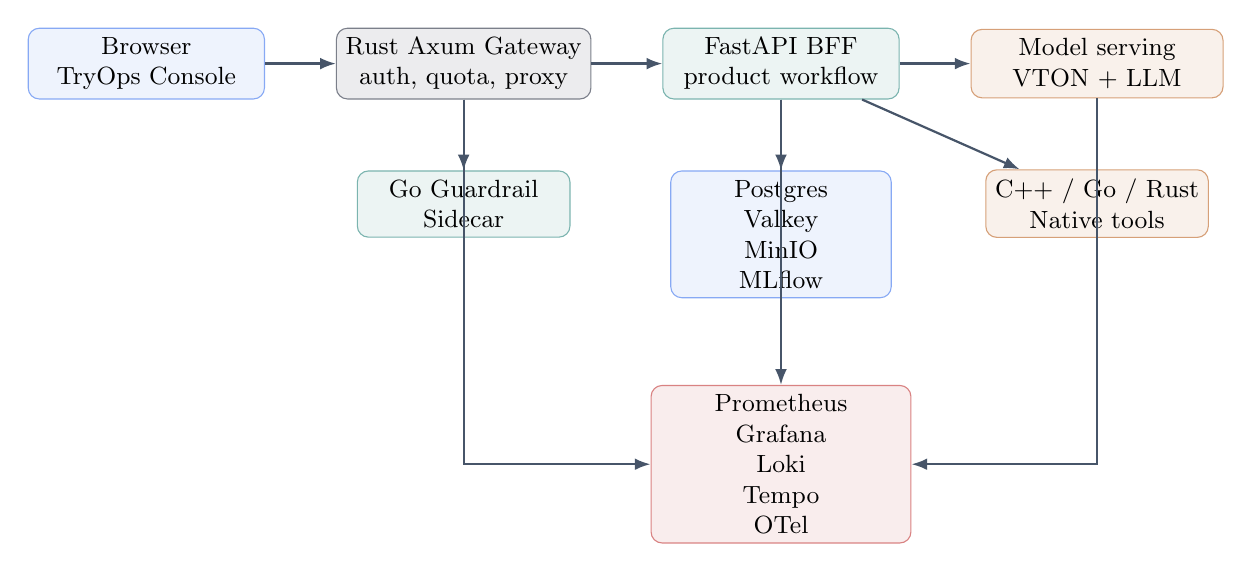
\begin{tikzpicture}[
  node distance=0.9cm and 0.9cm,
  box/.style={draw=#1!55, fill=#1!8, rounded corners=4pt, minimum height=0.8cm, align=center, font=\small},
  arrow/.style={-{Latex[length=2mm]}, thick, color=TryOpsSlate}
]
\node[box=TryOpsBlue, minimum width=3.0cm] (user) {Browser\\TryOps Console};
\node[box=TryOpsNavy, minimum width=3.1cm, right=of user] (gateway) {Rust Axum Gateway\\auth, quota, proxy};
\node[box=TryOpsTeal, minimum width=3.0cm, right=of gateway] (api) {FastAPI BFF\\product workflow};
\node[box=TryOpsGold, minimum width=3.2cm, right=of api] (models) {Model serving\\VTON + LLM};

\node[box=TryOpsTeal, minimum width=2.7cm, below=of gateway] (guardrail) {Go Guardrail\\Sidecar};
\node[box=TryOpsBlue, minimum width=2.8cm, below=of api] (data) {Postgres\\Valkey\\MinIO\\MLflow};
\node[box=TryOpsGold, minimum width=2.8cm, below=of models] (native) {C++ / Go / Rust\\Native tools};
\node[box=TryOpsRed, minimum width=3.3cm, below=1.1cm of data] (obs) {Prometheus\\Grafana\\Loki\\Tempo\\OTel};

\draw[arrow] (user) -- (gateway);
\draw[arrow] (gateway) -- (api);
\draw[arrow] (api) -- (models);
\draw[arrow] (gateway) -- (guardrail);
\draw[arrow] (api) -- (data);
\draw[arrow] (api) -- (native);
\draw[arrow] (gateway.south) |- (obs.west);
\draw[arrow] (api.south) -- (obs.north);
\draw[arrow] (models.south) |- (obs.east);
\end{tikzpicture}
\caption{Kiến trúc tổng quan của TryOps}
\end{figure}

\section{Lớp giao diện}

Thư mục \code{web/} chứa React/Vite console. Các component chính:

\begin{itemize}
  \item \code{VtonStudio.tsx}: upload ảnh, chọn category/source/quality, submit VTON job.
  \item \code{JobStatusList.tsx}: hiển thị job queued/running/completed/failed.
  \item \code{RecentTryOnGallery.tsx}: hiển thị output try-on gần đây.
  \item \code{LlmPlayground.tsx}: gửi prompt LLM.
  \item \code{AccountDashboardView.tsx}: quota, workspace, job slots.
  \item \code{DashboardView.tsx}, \code{GovernanceView.tsx}, \code{RegistryView.tsx}, \code{IncidentView.tsx}: operator/admin views.
  \item \code{auth.ts}: OIDC authorization-code + PKCE.
\end{itemize}

\section{Lớp Gateway}

Rust gateway trong \code{native/rust/tryops-gateway} là production-facing boundary:

\begin{itemize}
  \item Serve static UI.
  \item Proxy \code{/api/*} sang backend \code{/v1/*}.
  \item Validate API key hoặc JWT/OIDC.
  \item Enforce rate limit và payload limit.
  \item Enforce quota admission.
  \item Call Go guardrail sidecar trước LLM.
  \item Forward \code{traceparent} và request ID.
  \item Export Prometheus metrics.
  \item Hỗ trợ TLS profile.
\end{itemize}

Gateway giúp Python không trở thành điểm duy nhất chịu trách nhiệm cho edge security và quota.

\section{Lớp API/BFF}

\code{src/tryops/api.py} chứa FastAPI BFF. Vai trò:

\begin{itemize}
  \item VTON upload, infer, async jobs, account jobs.
  \item LLM generate.
  \item Account/session APIs.
  \item Artifact read/write.
  \item Dashboard rollups.
  \item Request history và feedback.
  \item Promotion/evaluation/governance endpoints.
  \item Observability recording.
\end{itemize}

FastAPI không trực tiếp quản lý worker GPU; nó gọi model serving qua URL ổn định.

\section{Lớp model serving}

\subsection{VTON}

Luồng hiện tại:

\begin{lstlisting}
API container
  -> TRYOPS_REAL_VTON_URL
  -> http://host.docker.internal:18100
  -> host FASHN router
  -> private worker Unix sockets
  -> CUDA GPU
\end{lstlisting}

Router trong \code{scripts/serve_fashn_vton_router.py}:

\begin{itemize}
  \item Sinh worker từ \code{TRYOPS_FASHN_GPU_IDS}.
  \item Pin mỗi worker bằng \code{CUDA_VISIBLE_DEVICES}.
  \item Dùng Unix socket mặc định để tránh public worker ports.
  \item Probe readiness từng worker.
  \item Route request theo least-inflight + round-robin giữa các worker ít tải.
  \item Export metrics có label \code{worker_id}, \code{gpu_id}, \code{gpu_uuid}, \code{status}.
  \item Ghi structured logs \code{fashn_vton_router_events.jsonl}.
\end{itemize}

\subsection{LLM}

LLM dùng OpenAI-compatible endpoint:

\begin{lstlisting}
TRYOPS_LLM_PROVIDER=openai_compatible
TRYOPS_LLM_BASE_URL=http://host.docker.internal:8000/v1
TRYOPS_LLM_MODEL=HuggingFaceTB/SmolLM2-135M-Instruct
\end{lstlisting}

Hoặc dùng OpenAI API:

\begin{lstlisting}
TRYOPS_LLM_BASE_URL=https://api.openai.com/v1
TRYOPS_LLM_MODEL=<model-name>
TRYOPS_LLM_API_KEY=<secret>
\end{lstlisting}

Adapter không có fallback. Nếu endpoint unreachable hoặc trả JSON sai contract, API nhận lỗi thật.

\section{Lớp dữ liệu và artifact}

\begin{longtable}{p{4cm}p{10.5cm}}
\toprule
\textbf{Thành phần} & \textbf{Vai trò} \\
\midrule
Postgres & Accounts, account members, requests, jobs, quota ledger, artifact metadata \\
Valkey & Hot counters cho quota/rate limit \\
MinIO & Object storage cho uploads, outputs, MLflow artifacts \\
MLflow & Tracking experiments và model evidence \\
DVC & Dataset/data versioning samples \\
\code{artifacts/} & Runtime logs, reports, model weights, generated outputs \\
\code{reports/generated/} & Promotion/evaluation evidence \\
\bottomrule
\end{longtable}

VTON upload đi qua \code{/api/vton/upload}, được chuẩn hóa thành PNG, lưu artifact và trả \code{artifact:<id>}.

\section{Lớp observability}

Các nguồn telemetry:

\begin{itemize}
  \item API metrics ở \code{/v1/metrics}.
  \item Gateway metrics ở \code{/metrics}.
  \item FASHN router metrics ở \code{/metrics}.
  \item Go guardrail metrics ở \code{/metrics}.
  \item Structured logs: \code{artifacts/logs/api_events.jsonl}, \code{fashn_vton_router_events.jsonl}, \code{fashn_vton_worker_*_events.jsonl}.
  \item Trace spans: \code{artifacts/traces/api_spans.jsonl}.
  \item OTel Collector + bridge gửi logs/traces tới Loki/Tempo.
\end{itemize}

Grafana dashboard:

\begin{itemize}
  \item \code{tryops-service-overview.json}
  \item \code{tryops-model-quality.json}
  \item \code{tryops-cost-capacity.json}
  \item \code{tryops-guardrails.json}
  \item \code{tryops-observability-drilldown.json}
\end{itemize}

% ---------------------------------------------------------------------------
\chapter{Thiết kế và triển khai các thành phần chính}
% ---------------------------------------------------------------------------

\section{TryOps Console}

TryOps Console là giao diện vận hành chính cho người dùng và operator. Giao diện không chỉ là demo upload/generate mà còn có các trang hỗ trợ MLOps:

\begin{itemize}
  \item Studio tạo VTON output.
  \item LLM Playground.
  \item Workspace/account dashboard.
  \item Request history.
  \item Registry và champion/challenger.
  \item Governance/lineage.
  \item Pipeline runs.
  \item Incidents và rollback evidence.
\end{itemize}

Điểm mạnh là UI đi qua API thật và gateway thật. Điểm còn hạn chế là một số view vẫn cần hoàn thiện click-through lineage, export và accessibility.

\section{Xác thực, tài khoản và quota}

TryOps sử dụng Keycloak làm OIDC provider. Browser thực hiện login/signup qua PKCE; gateway validate token trước khi forward principal metadata vào FastAPI. Khi user đăng nhập lần đầu, API bootstrap workspace account trong Postgres.

Quota được áp dụng ở hai mức:

\begin{itemize}
  \item Rust Gateway: quota/rate admission cho request edge.
  \item FastAPI: workload-level quota và VTON workspace concurrency.
\end{itemize}

VTON job concurrency mặc định:

\begin{center}
\begin{tabular}{lr}
\toprule
\textbf{Plan} & \textbf{Active VTON jobs} \\
\midrule
free & 1 \\
team & 2 \\
enterprise & 4 \\
\bottomrule
\end{tabular}
\end{center}

Các biến override:

\begin{lstlisting}
TRYOPS_VTON_CONCURRENCY_FREE=1
TRYOPS_VTON_CONCURRENCY_TEAM=2
TRYOPS_VTON_CONCURRENCY_ENTERPRISE=4
TRYOPS_VTON_JOB_WORKERS=1
\end{lstlisting}

Điểm cần lưu ý: plan limit là số job active theo workspace; \code{TRYOPS_VTON_JOB_WORKERS} là số worker job trong API queue. Chúng không đồng nghĩa với số GPU worker phía FASHN router.

\section{VTON async job lifecycle}

Luồng VTON:

\begin{enumerate}
  \item User upload person image và garment image.
  \item API lưu ảnh thành artifact.
  \item User submit VTON job.
  \item API kiểm tra payload, auth, quota, concurrency.
  \item \code{VTON_JOB_QUEUE} nhận job và persist snapshot.
  \item Runner gọi \code{_vton_infer_impl}.
  \item Adapter gọi FASHN router qua \code{TRYOPS_REAL_VTON_URL}.
  \item FASHN worker sinh output PNG và report.
  \item API persist request record và job result.
  \item UI poll job status và mở output artifact.
\end{enumerate}

Các trạng thái chính:

\begin{center}
\begin{tabular}{ll}
\toprule
\textbf{Status} & \textbf{Ý nghĩa} \\
\midrule
accepted & API đã nhận job \\
queued & job trong hàng chờ \\
running & job đang chạy \\
completed & job hoàn tất, có output \\
failed & job thất bại, có error \\
\bottomrule
\end{tabular}
\end{center}

\section{FASHN multi-GPU router}

Router là abstraction quan trọng nhất để không hardcode worker ports/GPU trong API.

Biến cấu hình local:

\begin{lstlisting}
TRYOPS_REAL_VTON_URL=http://host.docker.internal:18100
TRYOPS_FASHN_GPU_IDS=0,1,2
TRYOPS_FASHN_WORKER_TRANSPORT=unix
TRYOPS_FASHN_WORKER_SOCKET_DIR=artifacts/runtime/fashn-workers
TRYOPS_FASHN_WORKER_PRELOAD=1
TRYOPS_FASHN_REQUIRE_CUDA=1
TRYOPS_FASHN_ALLOW_CPU_FALLBACK=0
\end{lstlisting}

Router sinh worker:

\begin{center}
\begin{tabular}{lll}
\toprule
\textbf{Worker} & \textbf{CUDA pin} & \textbf{Endpoint nội bộ} \\
\midrule
\code{fashn-gpu0} & \code{CUDA_VISIBLE_DEVICES=0} & Unix socket \\
\code{fashn-gpu1} & \code{CUDA_VISIBLE_DEVICES=1} & Unix socket \\
\code{fashn-gpu2} & \code{CUDA_VISIBLE_DEVICES=2} & Unix socket \\
\bottomrule
\end{tabular}
\end{center}

Prometheus chỉ cần scrape router \code{/metrics}, không cần biết từng worker port. Grafana có thể vẽ per-worker throughput, latency, in-flight và failure bằng metric labels.

\section{LLM real endpoint}

LLM adapter chính gọi \code{/chat/completions} theo OpenAI-compatible schema. Adapter ghi:

\begin{itemize}
  \item model name/provider/base URL đã sanitize,
  \item input/output token count,
  \item latency,
  \item tokens/sec,
  \item cost estimate theo env,
  \item safety flags,
  \item structured answer nếu yêu cầu.
\end{itemize}

Khi không có endpoint thật, lỗi được surface lên caller. Đây là hành vi đúng cho production vì không đánh lừa người dùng bằng deterministic response.

\section{Guardrails}

Guardrail triển khai ở gateway và API:

\begin{itemize}
  \item Chặn prompt injection.
  \item Chặn system prompt leakage.
  \item Mask PII/secret-like strings.
  \item Giới hạn unbounded output.
  \item Validate structured output.
  \item Export metrics theo OWASP LLM risk.
\end{itemize}

Go sidecar nằm ở \code{native/go/tryops-guardrail}, Docker Compose chạy service \code{guardrail}. Gateway gọi qua \code{TRYOPS_GATEWAY_GUARDRAIL_URL}; API gọi qua \code{TRYOPS_GUARDRAIL_URL}.

\section{Governance và promotion gate}

Model promotion yêu cầu các artifact:

\begin{itemize}
  \item model card,
  \item data card,
  \item evaluation report,
  \item SBOM,
  \item model artifact scan,
  \item provenance attestation,
  \item risk controls,
  \item owner approvals,
  \item policy verdict.
\end{itemize}

State của model:

\begin{center}
\begin{tabular}{ll}
\toprule
\textbf{State} & \textbf{Ý nghĩa} \\
\midrule
candidate & mới sinh từ pipeline, chưa tin cậy \\
challenger & đã qua staging gate, có thể shadow/canary \\
champion & model production-demo \\
rejected & bị chặn bởi policy \\
archived & giữ để truy vết \\
\bottomrule
\end{tabular}
\end{center}

Các tool liên quan:

\begin{itemize}
  \item Python policy: \code{src/tryops/policy.py}
  \item C++ policy CLI: \code{artifacts/native/tryops_policy_cli}
  \item Go controller: \code{native/go/tryops-controller}
  \item Supply chain: \code{docs/supply_chain.md}, \code{configs/model_sources.json}, \code{configs/dataset_licenses.json}
\end{itemize}

\section{Native production boundary}

TryOps cố ý không đặt toàn bộ production boundary vào Python.

\begin{longtable}{p{3cm}p{11.5cm}}
\toprule
\textbf{Runtime} & \textbf{Vai trò} \\
\midrule
Rust & Gateway, auth, quota, rate limit, proxy, metrics, TLS, static serving \\
Go & Guardrail, controller, event dispatcher, job runner, load driver, contracts \\
C++ & Policy, perf stats, image metrics, VTON preprocess/eval, energy, cache, model scan \\
Python & BFF, ML adapters, orchestration, evaluation helpers \\
\bottomrule
\end{longtable}

Mô hình này giúp các quyết định performance/risk-critical có thể chạy ở runtime biên có kiểm soát hơn.

% ---------------------------------------------------------------------------
\chapter{Thực nghiệm và đánh giá}
% ---------------------------------------------------------------------------

\section{Kiểm thử và evidence trong repo}

Repo có hệ thống test và Make targets rộng:

\begin{itemize}
  \item Python tests trong \code{tests/}.
  \item Web typecheck/build: \code{make web-typecheck}, \code{make web-build}.
  \item Rust: \code{make native-rust-test}, \code{make native-rust-smoke}.
  \item Go: \code{make native-go-test}, \code{make native-go-smoke}.
  \item C++: \code{make native-cpp-test}.
  \item Full product: \code{make app-up}, \code{make app-smoke}, \code{make app-down}.
  \item VTON: \code{make fashn-vton-sample}, \code{make benchmark-vton}.
  \item LLM: \code{make llm-vllm-probe-sample}, \code{make llm-pareto-sample}.
  \item Observability: \code{make dashboard-sample}, \code{make trace-sample}, \code{make alert-sample}.
  \item Governance: \code{make governance-sample}, \code{make model-supply-chain-sample}.
\end{itemize}

Trong quá trình viết báo cáo này, nhóm không chạy lại full test vì một số mục có thể kích hoạt GPU/model inference nặng; báo cáo dựa trên code, docs, slide và artifact paths đã có.

\section{Kết quả VTON benchmark từ slide}

Slide \code{slide/main.tex} ghi nhận bảng so sánh VTON:

\begin{longtable}{p{3.3cm}rrrrrrrr}
\toprule
\textbf{Dataset / Target} & \textbf{SSIM} & \textbf{PSNR} & \textbf{Avg ms} & \textbf{P95 ms} & \textbf{req/s} & \textbf{Model ms} & \textbf{GPU \%} & \textbf{VRAM GB} \\
\midrule
FASHN VTON v1.5 & 0.888121 & 18.915 & 21,337.50 & 23,244.00 & 0.045439 & 19,969.60 & 100.00 & 4.825 \\
CatVTON & 0.861734 & 18.284 & 17,842.30 & 19,604.00 & 0.054261 & 16,512.80 & 96.50 & 6.742 \\
IDM-VTON & 0.879462 & 18.671 & 42,586.70 & 47,918.00 & 0.022751 & 40,318.40 & 99.20 & 13.684 \\
OOTDiffusion & 0.852918 & 17.936 & 35,214.90 & 39,876.00 & 0.027502 & 33,087.60 & 98.40 & 10.927 \\
\bottomrule
\end{longtable}

Nhận xét:

\begin{itemize}
  \item FASHN VTON v1.5 có SSIM/PSNR cao nhất trong bảng và VRAM thấp nhất.
  \item CatVTON có latency/throughput tốt nhất nhưng chất lượng thấp hơn FASHN trong bảng này.
  \item IDM-VTON và OOTDiffusion nặng hơn về latency, VRAM và RAM.
  \item FASHN là lựa chọn hợp lý cho production-local stack nếu mục tiêu là chất lượng ảnh và VRAM vừa phải.
\end{itemize}

\section{Đánh giá balancer VTON}

Router FASHN export metric:

\begin{lstlisting}
tryops_fashn_router_worker_requests_total{worker_id="...",gpu_id="...",status="completed"}
tryops_fashn_router_worker_inflight{worker_id="...",gpu_id="..."}
tryops_fashn_router_latency_ms_count
tryops_fashn_router_latency_ms_sum
\end{lstlisting}

Để stress test balancer, repo có helper shell trong \code{artifacts/tools/stress_vton_balancer.sh} gọi trực tiếp router, bắn nhiều request cùng lúc và so sánh metrics trước/sau. Kỳ vọng khi \code{TRYOPS_FASHN_GPU_IDS=0,1,2} là request delta phân bố trên \code{fashn-gpu0}, \code{fashn-gpu1}, \code{fashn-gpu2}.

\section{LLM evaluation}

Repo có hai loại LLM evidence:

\begin{enumerate}
  \item Baseline/harness evidence cho kiểm thử contract và evaluation pipeline.
  \item Real serving path qua OpenAI-compatible endpoint.
\end{enumerate}

Tài liệu \code{docs/llm_vllm.md} ghi nhận native Go vLLM probe có thể kiểm tra:

\begin{itemize}
  \item GPU availability,
  \item \code{vllm} binary,
  \item \code{/v1/models},
  \item \code{/v1/chat/completions},
  \item \code{/metrics},
  \item bounded concurrent load probe.
\end{itemize}

Nếu không có vLLM endpoint live ở \code{127.0.0.1:8000/v1}, report sẽ ghi \code{status=skipped}. Đây là readiness evidence, không phải benchmark giả. Với OpenAI API, endpoint thật nằm ngoài máy local và cần \code{TRYOPS_LLM_API_KEY}.

\section{Observability evaluation}

Các dashboard Grafana đã được provision:

\begin{longtable}{p{5cm}p{9.8cm}}
\toprule
\textbf{Dashboard} & \textbf{Mục tiêu} \\
\midrule
TryOps Service Overview & request rate, error ratio, latency, memory, queue depth, gateway errors \\
TryOps Model Quality & quality score, VTON latency, LLM throughput, completed inference \\
TryOps Cost and Capacity & cost, quota utilization, semantic-cache hit, energy/carbon \\
TryOps Guardrails & blocked/redacted/reviewed findings theo OWASP risk \\
TryOps Observability Drilldown & logs, job lifecycle, FASHN service logs, OTel/Tempo/Loki health \\
\bottomrule
\end{longtable}

Điểm quan trọng là Grafana không chỉ xem CPU/RAM; nó phải giúp debug request-level model failures bằng \code{request_id} và \code{job_id}.

\section{Đánh giá vận hành}

Kết quả thiết kế vận hành:

\begin{itemize}
  \item \code{make app-up} khởi động cả product stack và FASHN router.
  \item \code{keycloak-db-init} exited là trạng thái đúng vì đó là init job một lần.
  \item \code{make app-down} dừng compose và router; nếu container zombie, cần Docker/init handling.
  \item Grafana ở \code{127.0.0.1:13000}.
  \item Loki logs API ở \code{127.0.0.1:13100}.
  \item Tempo traces API ở \code{127.0.0.1:13200}.
  \item OTel bridge metrics ở \code{127.0.0.1:19122/metrics}.
\end{itemize}

% ---------------------------------------------------------------------------
\chapter{Triển khai, vận hành và giám sát}
% ---------------------------------------------------------------------------

\section{Cách chạy local}

Chuẩn bị \code{.env} từ \code{.env.example}, sau đó:

\begin{lstlisting}
make app-up
\end{lstlisting}

Mở console:

\begin{lstlisting}
http://127.0.0.1:18081
\end{lstlisting}

Kiểm tra health:

\begin{lstlisting}
curl -fsS http://127.0.0.1:18081/api/health
make app-smoke
\end{lstlisting}

Dừng hệ thống:

\begin{lstlisting}
make app-down
\end{lstlisting}

\section{Biến môi trường production-critical}

\begin{longtable}{p{5.7cm}p{9cm}}
\toprule
\textbf{Biến} & \textbf{Ý nghĩa} \\
\midrule
\code{TRYOPS_REQUIRE_REAL_MODELS=1} & Bắt buộc endpoint model thật \\
\code{TRYOPS_ALLOW_DETERMINISTIC_BASELINE=0} & Không cho baseline như product \\
\code{TRYOPS_LLM_BASE_URL} & OpenAI-compatible endpoint \\
\code{TRYOPS_LLM_MODEL} & Model LLM thật \\
\code{TRYOPS_LLM_API_KEY} & Secret key nếu dùng provider cần auth \\
\code{TRYOPS_REAL_VTON_URL} & FASHN router URL \\
\code{TRYOPS_FASHN_GPU_IDS} & GPU list cho router sinh worker \\
\code{TRYOPS_FASHN_REQUIRE_CUDA=1} & Bắt buộc CUDA \\
\code{TRYOPS_FASHN_ALLOW_CPU_FALLBACK=0} & Không fallback CPU \\
\code{TRYOPS_ENABLE_LOCAL_API_KEYS=0} & Tắt static dev keys \\
\code{TRYOPS_ENABLE_DEV_API_KEY_FALLBACK=0} & Tắt dev fallback \\
\bottomrule
\end{longtable}

\section{Port surface local}

Các port chính trong developer-local mode:

\begin{longtable}{p{5.5cm}p{9.2cm}}
\toprule
\textbf{Service} & \textbf{URL/Port} \\
\midrule
Console + Rust gateway & \code{http://127.0.0.1:18081} \\
Keycloak & \code{http://127.0.0.1:18082} \\
Grafana & \code{http://127.0.0.1:13000} \\
FASHN router & \code{http://127.0.0.1:18100} \\
FastAPI direct & \code{http://127.0.0.1:18080} \\
MinIO API/Console & \code{19000} / \code{19001} \\
MLflow & \code{15000} \\
Prometheus & \code{19090} \\
Loki & \code{13100} \\
Tempo & \code{13200} \\
\bottomrule
\end{longtable}

\code{PORT.md} nhấn mạnh đây là developer-local convenience surface, không phải shared datacenter posture.

\section{Shared datacenter design}

Thiết kế khuyến nghị cho máy dùng chung:

\begin{lstlisting}
users/operators
  -> ingress/reverse proxy
      -> gateway / console
      -> keycloak
      -> grafana

internal network only
  -> api, postgres, valkey, minio, mlflow
  -> prometheus, loki, tempo, alertmanager, otel
  -> guardrail
  -> fashn router / workers
  -> optional vLLM
\end{lstlisting}

Nếu chưa có ingress/DNS, chỉ nên expose:

\begin{center}
\begin{tabular}{ll}
\toprule
\textbf{Port} & \textbf{Service} \\
\midrule
\code{18081} & gateway / console \\
\code{18082} & Keycloak \\
\code{13000} & Grafana \\
\bottomrule
\end{tabular}
\end{center}

Không nên expose worker ports, database ports, MinIO, Prometheus, Loki, Tempo hoặc model endpoints ra cho người dùng khác trên datacenter.

\section{Giám sát logs trong Grafana}

Với \code{TRYOPS_OBSERVABILITY=1}, \code{make app-up} chạy Loki, Tempo, OTel collector và OTel bridge. Trong Grafana:

\begin{enumerate}
  \item Mở \code{http://127.0.0.1:13000}.
  \item Vào dashboard \textbf{TryOps Observability Drilldown}.
  \item Xem các panel: FASHN VTON Service Logs, Async Job Lifecycle Logs, Error Logs, API/gateway runtime metrics.
  \item Dùng \code{job_id} hoặc \code{request_id} để correlate UI job với API logs và FASHN router/worker logs.
\end{enumerate}

Raw log paths:

\begin{lstlisting}
artifacts/logs/api_events.jsonl
artifacts/logs/fashn-vton-router.log
artifacts/logs/fashn_vton_router_events.jsonl
artifacts/logs/fashn-vton-worker-*.log
artifacts/logs/fashn_vton_worker_*_events.jsonl
\end{lstlisting}

\section{Custom hostname và browser auth}

Không nên dùng plain HTTP với hosts-file domain như:

\begin{lstlisting}
http://tryops.com:18081
\end{lstlisting}

Lý do: OIDC PKCE cần \code{crypto.subtle.digest}, chỉ có trên HTTPS hoặc trusted loopback origin như \code{localhost}/\code{127.0.0.1}. Nếu cần vanity hostname, phải cấu hình HTTPS, cert SAN, Keycloak redirect URI và public issuer phù hợp.

% ---------------------------------------------------------------------------
\chapter{Bảo mật, quản trị mô hình và trách nhiệm AI}
% ---------------------------------------------------------------------------

\section{Xác thực và phân quyền}

TryOps dùng Keycloak/OIDC cho login. Gateway validate token và forward principal metadata. Local static API keys tồn tại cho debug nhưng mặc định bị tắt trong \code{.env.example}.

Các role và quyền liên quan:

\begin{itemize}
  \item viewer,
  \item operator,
  \item admin,
  \item account roles,
  \item promotion/admin scopes.
\end{itemize}

\section{Bảo vệ dữ liệu người dùng}

Ảnh upload là dữ liệu nhạy cảm. Hệ thống áp dụng:

\begin{itemize}
  \item Không đưa raw image content vào log.
  \item Artifact storage qua MinIO/local runtime artifacts.
  \item Metadata gồm role, content type, width/height, request ID, account ID.
  \item Dataset license inventory phân biệt user-uploaded images và benchmark datasets.
\end{itemize}

\section{Guardrails cho LLM}

LLM guardrail map vào OWASP LLM 2025:

\begin{longtable}{p{3cm}p{11.5cm}}
\toprule
\textbf{OWASP ID} & \textbf{Control} \\
\midrule
LLM01 & Prompt injection classifier \\
LLM02 & PII/secret disclosure masking/blocking \\
LLM05 & Structured output validation \\
LLM06 & Unsafe agency classifier \\
LLM07 & System prompt leakage detection \\
LLM10 & Unbounded output / max-token guard \\
\bottomrule
\end{longtable}

Gateway và API đều có vị trí kiểm tra để tránh chỉ dựa vào model output.

\section{Supply chain}

Supply-chain evidence bao gồm:

\begin{itemize}
  \item \code{uv.lock}, \code{web/package-lock.json}, Rust \code{Cargo.lock}, Go \code{go.sum}.
  \item SBOM SPDX.
  \item Model source pins.
  \item Dataset license inventory.
  \item SafeTensors-only model scan.
  \item Provenance attestation.
  \item Trivy/Syft/Cosign CI contract.
  \item GitHub Actions workflow.
\end{itemize}

Rủi ro còn lại: production Sigstore/Rekor transparency, external secret sync, scanner coverage mở rộng.

\section{Governance và policy gate}

Một model không được promotion nếu thiếu:

\begin{itemize}
  \item evaluation report,
  \item model/data card,
  \item SBOM,
  \item scan/provenance,
  \item owner approval,
  \item risk status,
  \item passing metrics,
  \item no high/critical vulnerabilities.
\end{itemize}

Một candidate bị chặn là kết quả đúng của production governance, không phải lỗi demo.

% ---------------------------------------------------------------------------
\chapter{Hạn chế hiện tại và hướng phát triển}
% ---------------------------------------------------------------------------

\section{Hạn chế hiện tại}

\begin{longtable}{p{4cm}p{5.5cm}p{5.2cm}}
\toprule
\textbf{Hạn chế} & \textbf{Bằng chứng trong repo} & \textbf{Hướng xử lý} \\
\midrule
UI VTON job sau refresh vẫn đang fetch/filter active jobs & \code{web/src/App.tsx} gọi \code{accountJobs("active", 20)}, \code{VtonStudio.tsx} filter \code{isActiveVtonJob} & Fetch recent/all jobs, tách active slot count khỏi visible history \\
Shared datacenter mode mới là plan/docs, chưa là compose profile hoàn chỉnh & \code{docs/shared_datacenter_networking_plan.md}, \code{PORT.md} & Tạo \code{docker-compose.shared.yml}, chỉ expose ingress/gateway/auth/Grafana \\
GPU/process exporters chưa đầy đủ & \code{docs/multi_gpu_fashn_serving_plan.md} ghi remaining work & Thêm DCGM exporter, node exporter, process exporter và Grafana panels \\
vLLM live benchmark phụ thuộc endpoint đang chạy & \code{docs/llm_vllm.md} ghi skipped nếu không có vLLM & Đóng gói vLLM profile hoặc dùng OpenAI endpoint có key \\
Keycloak custom domain cần HTTPS & \code{PORT.md} browser auth section & TLS profile, redirect URI, public issuer và cert SAN \\
Production Kubernetes/External Secrets chưa hoàn chỉnh & \code{docs/production_app_plan.md} & Vault/External Secrets operator sync trong cluster \\
VTON fairness/human preference chưa đại diện & \code{docs/vton_results.md} & Thu thập panel người dùng và benchmark dataset hợp lệ \\
\bottomrule
\end{longtable}

\section{Hướng phát triển}

\begin{enumerate}
  \item Hoàn thiện job history UI để completed/failed jobs không biến mất sau F5.
  \item Đóng gói shared datacenter compose/ingress mode.
  \item Thêm GPU hardware telemetry vào Grafana: DCGM, power, VRAM, utilization, worker process.
  \item Thêm load test chính thức cho router/API/jobs bằng native Go hoặc shell helper chuẩn hóa.
  \item Hoàn thiện OpenTelemetry live exporters từ mọi runtime.
  \item Hoàn thiện runbook vận hành production.
  \item Tích hợp KServe/vLLM cho cluster-grade serving.
  \item Hoàn thiện external secrets, rotation và backup/restore production drills.
  \item Bổ sung human evaluation cho VTON quality/fairness.
  \item Chuẩn hóa report artifact xuất PDF/HTML từ Markdown hoặc LaTeX.
\end{enumerate}

% ---------------------------------------------------------------------------
\chapter{Kết luận}
% ---------------------------------------------------------------------------

TryOps chứng minh rằng một đồ án MLOps production-minded phải vượt khỏi phạm vi ``model + UI demo''. Hệ thống hiện có một stack chạy được, có sản phẩm web, gateway native, API BFF, real VTON router, real LLM endpoint contract, account/quota, artifact storage, observability, governance, supply-chain evidence và nhiều native tools.

Điểm quan trọng nhất của TryOps là tính trung thực kỹ thuật: production path không âm thầm fallback sang mock/baseline. Nếu real LLM endpoint hoặc FASHN VTON router không sẵn sàng, hệ thống phải trả lỗi thật để operator sửa hạ tầng. Baseline tồn tại để kiểm thử, chẩn đoán, so sánh và giảng giải MLOps contract, không phải để bán như năng lực AI thật.

Với các phần còn lại như shared datacenter mode, GPU exporters, job history UI và cluster-grade serving, TryOps đã có hướng phát triển rõ ràng. Vì vậy, đóng góp chính của đồ án là một nền tảng MLOps có tư duy sản xuất: mô hình phải có bằng chứng, phải qua policy gate, phải có observability, phải truy vết được và phải fail-closed khi phụ thuộc thật không sẵn sàng.

% ---------------------------------------------------------------------------
\chapter*{Tài liệu và mã nguồn tham khảo}
\addcontentsline{toc}{chapter}{Tài liệu và mã nguồn tham khảo}
% ---------------------------------------------------------------------------

\section*{Tài liệu nội bộ trong repo}

\begin{itemize}
  \item \code{README.md} -- hướng dẫn chạy, kiến trúc và real VTON model.
  \item \code{PORT.md} -- port inventory, shared datacenter policy và browser auth caveats.
  \item \code{MLOPS_VTON_LLM_ENTERPRISE_ROADMAP.md} -- roadmap tổng thể.
  \item \code{reports/final_report.md} -- draft report cũ.
  \item \code{slide/main.tex}, \code{slide/main.pdf} -- slide bảo vệ.
  \item \code{docs/project_charter.md} -- thesis, motivation, users, success criteria.
  \item \code{docs/architecture.md} -- kiến trúc local/enterprise.
  \item \code{docs/production_app_plan.md} -- kế hoạch product stack.
  \item \code{docs/multi_gpu_fashn_serving_plan.md} -- thiết kế FASHN multi-GPU router.
  \item \code{docs/shared_datacenter_networking_plan.md} -- thiết kế port surface cho shared host.
  \item \code{docs/observability_contract.md} -- metrics/logs/traces contract.
  \item \code{docs/dashboard_design.md} -- Grafana dashboards.
  \item \code{docs/vton_job_persistence_and_readiness_plan.md} -- phân tích bug job visibility/readiness.
  \item \code{docs/vton_results.md} -- VTON baseline/eval evidence.
  \item \code{docs/llm_vllm.md}, \code{docs/llm_results.md}, \code{docs/llm_guardrails.md} -- LLM serving và guardrails.
  \item \code{docs/model_governance.md}, \code{docs/supply_chain.md}, \code{docs/enterprise_quota.md} -- governance, supply chain, quota.
\end{itemize}

\section*{Mã nguồn chính}

\begin{itemize}
  \item \code{web/src/} -- TryOps Console.
  \item \code{native/rust/tryops-gateway/} -- Rust Gateway.
  \item \code{src/tryops/api.py} -- FastAPI BFF.
  \item \code{src/tryops/pipelines/vton_remote.py} -- real FASHN VTON adapter.
  \item \code{src/tryops/pipelines/llm_openai_compatible.py} -- real LLM adapter.
  \item \code{scripts/serve_fashn_vton_router.py} -- host-side FASHN router.
  \item \code{scripts/serve_fashn_vton.py} -- FASHN worker service.
  \item \code{native/go/tryops-guardrail/} -- guardrail sidecar.
  \item \code{native/go/tryops-controller/} -- promotion/controller service.
  \item \code{native/cpp/} -- native C++ policy/metrics/eval tools.
  \item \code{infra/grafana/dashboards/} -- dashboard JSON.
  \item \code{infra/prometheus/} -- scrape configs và alert rules.
  \item \code{infra/otel/}, \code{infra/loki/}, \code{infra/tempo/} -- observability stack.
  \item \code{docker-compose.yml}, \code{docker-compose.observability.yml}, \code{Makefile}, \code{.env.example}.
\end{itemize}

% ---------------------------------------------------------------------------
\appendix
\chapter{Lệnh vận hành}
% ---------------------------------------------------------------------------

\section{Chạy stack}

\begin{lstlisting}
cp .env.example .env
make app-up
\end{lstlisting}

Console:

\begin{lstlisting}
http://127.0.0.1:18081
\end{lstlisting}

Grafana:

\begin{lstlisting}
http://127.0.0.1:13000
\end{lstlisting}

Stop:

\begin{lstlisting}
make app-down
\end{lstlisting}

\section{Kiểm tra FASHN router}

\begin{lstlisting}
make fashn-vton-workers-status
curl -fsS http://127.0.0.1:18100/ready
curl -fsS http://127.0.0.1:18100/metrics
\end{lstlisting}

Stress balancer:

\begin{lstlisting}
COUNT=10 TIMESTEPS=30 artifacts/tools/stress_vton_balancer.sh
\end{lstlisting}

\section{Chạy LLM thật bằng vLLM hoặc OpenAI-compatible endpoint}

\begin{lstlisting}
vllm serve HuggingFaceTB/SmolLM2-135M-Instruct --host 127.0.0.1 --port 8000
TRYOPS_LLM_BASE_URL=http://host.docker.internal:8000/v1 make app-up
\end{lstlisting}

Hoặc dùng OpenAI-compatible provider:

\begin{lstlisting}
TRYOPS_LLM_BASE_URL=https://api.openai.com/v1
TRYOPS_LLM_MODEL=<model-name>
TRYOPS_LLM_API_KEY=<secret>
\end{lstlisting}

Không commit secret vào repo.

\section{Observability}

\begin{lstlisting}
make dashboard-sample
make trace-sample
make alert-sample
\end{lstlisting}

Log paths:

\begin{lstlisting}
artifacts/logs/api_events.jsonl
artifacts/logs/fashn_vton_router_events.jsonl
artifacts/logs/fashn_vton_worker_*_events.jsonl
\end{lstlisting}

\section{Governance và supply chain}

\begin{lstlisting}
make governance-sample
make supply-chain-sample
make model-supply-chain-sample
make native-dependency-lock-contract-sample
\end{lstlisting}

\section{Kiểm thử}

\begin{lstlisting}
make test
make web-typecheck
make native-rust-test
make native-go-test
make native-cpp-test
\end{lstlisting}

% ---------------------------------------------------------------------------
\chapter{Checklist production truthfulness}
% ---------------------------------------------------------------------------

\begin{longtable}{p{6cm}p{8.5cm}}
\toprule
\textbf{Câu hỏi} & \textbf{Trạng thái hiện tại} \\
\midrule
Có default dùng real model không? & Có, \code{.env.example} yêu cầu real models và tắt baseline \\
VTON real adapter có fallback không? & Không, \code{vton_remote.py} raise \code{RealVtonUnavailableError} \\
LLM real adapter có fallback không? & Không, \code{llm_openai_compatible.py} raise \code{RealLLMUnavailableError} \\
Baseline có bị bán như production không? & Không nên; báo cáo này ghi baseline là diagnostics/offline harness \\
Local static API key có bật mặc định không? & Không, \code{.env.example} tắt local/dev fallback keys \\
Worker GPU ports có hardcode vào API không? & Không, API chỉ biết \code{TRYOPS_REAL_VTON_URL} \\
Grafana có xem logs/job/model-service không? & Có dashboard drilldown, Loki/OTel bridge trong local stack \\
Có known limitation rõ ràng không? & Có, Chương 8 liệt kê hạn chế hiện tại \\
\bottomrule
\end{longtable}

\end{document}
